\section{Auswertung}
\label{sec:Auswertung}
\subsection{Statische Methode}

In den Abbildungen \ref{abb:T1T4} und \ref{abb:T5T8} ist der
Temperatur Verlauf sowohl an den Punkten $T_1$ und $T_4$ als
auch den Punkten $T_5$ und $T_8$dargestellt die in der Abbildung
\ref{abb:Aufbau} zu finden sind.


\begin{figure}
  \centering
  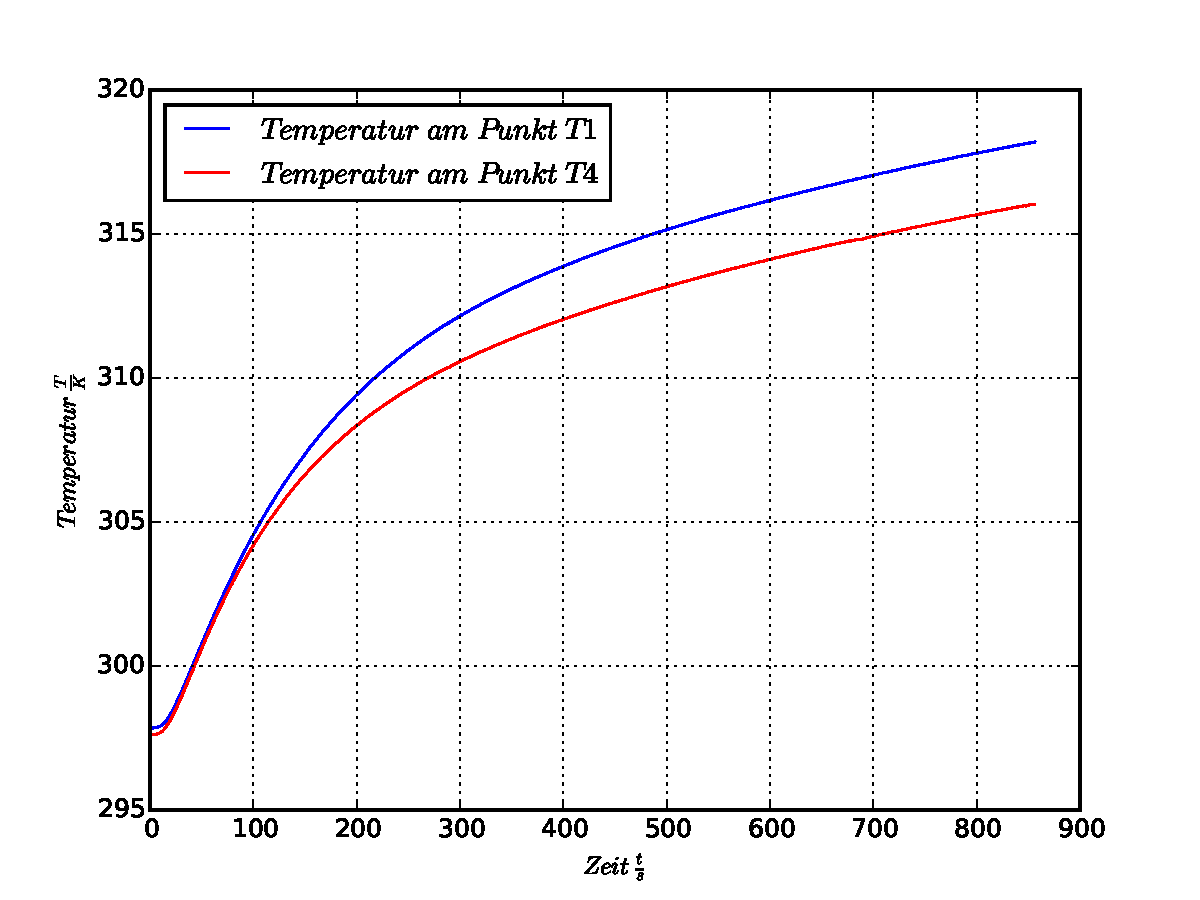
\includegraphics[width=0.7\textwidth]{plotT1T4.pdf}
  \caption{Temperaturverlauf am Punkt T1 und T4.}
  \label{abb:T1T4}
  \end{figure}
\begin{figure}
    \centering
    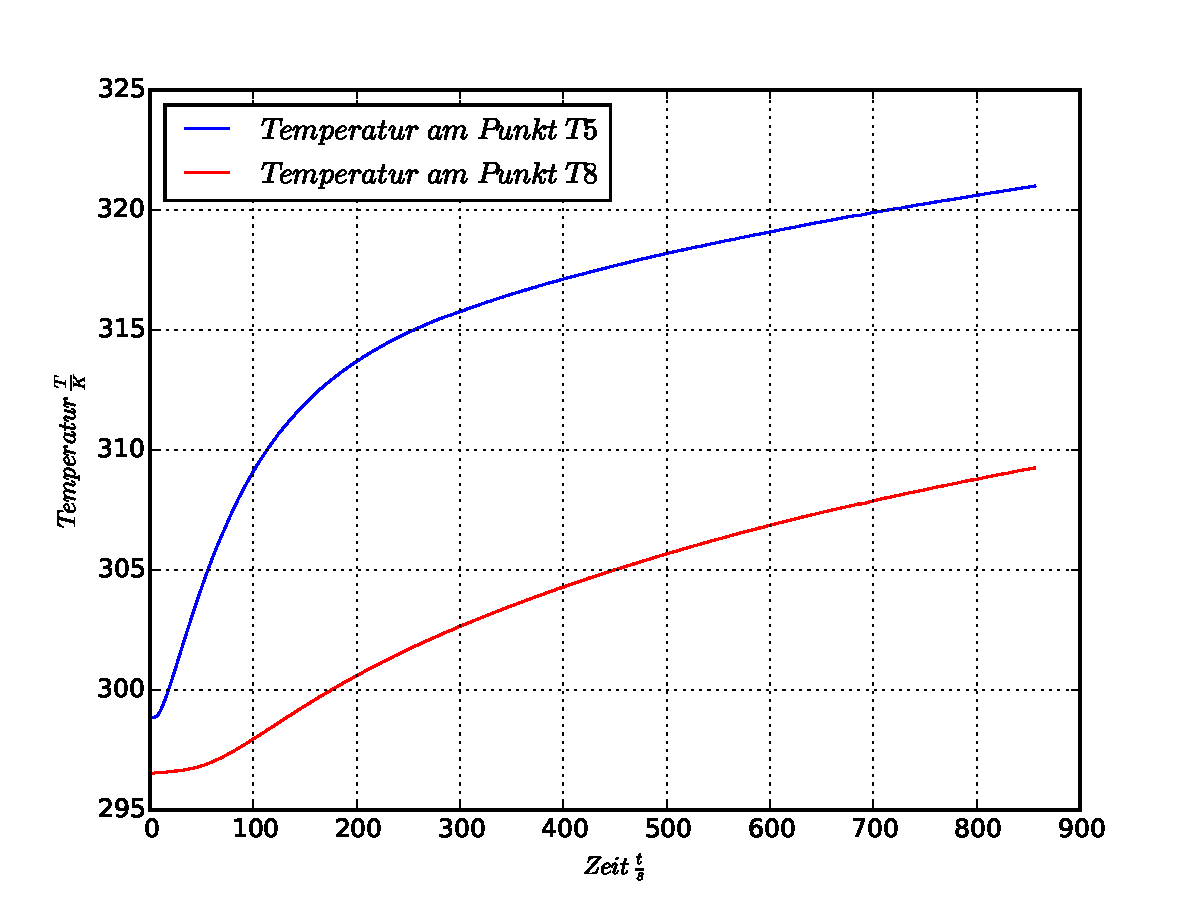
\includegraphics[width=0.7\textwidth]{plotT5T8.pdf}
    \caption{Temperaturverlauf am Punkt T5 und T8.}
    \label{abb:T5T8}
\end{figure}
Die vier Kurven die in den
Abbildungen \ref{abb:T1T4} und \ref{abb:T5T8}
zusehen sind besitzten alle einen ähnlichen Verlauf.
Am Anfang ist die Temperatur kurz konstant
ehe sie schnell steigt. In der Mitte begint
sich die Steigung sich wieder zu verringern,
bis sich am Ende  eine fast konstante
Steigung einstellt. Nur die Kurve von dem Punkt 8 besitzt
zu Begin keine starke Steigung sondern steigt eher langsam
an.



Desweiteren lässt sich eine Aussage über die Wärmeleitfähigkeit
der Materialien machen, indem die Temperatur zu einem
bestimmten Zeitpunkt\footnote{hier nach $700\,\si{second}$}
von den  fernen Thermoelementen verglichen wird.
Welches  Thermoelement die höchste Temperatur zu diesem Zeitpunkt
anzeigt, besitzt die größe Wärmeleitfähigkeit
da alle Thermoelemente  gleich weit von dem
Peletiereelement entfernt sind und alle bei Raumtemperatur
starten.
Aus den Messwerte
\begin{align*}
T_1=43,89\,\si{\kelvin},\\
T_4=41,78\,\si{\kelvin},\\
T_5=46,75\,\si{\kelvin},\\
T_8=34,73\,\si{\kelvin}
\end{align*}
kann vermutet werden, dass der Aluminiumstab
die höchste Wärmeleitfähigkeit besitzt.
Danach folgt der breite Messingstab, dann der schmale Messingstab
und die geringste Wärmeleitfähigkeit besitzt somit der Edelstahlstab.

Ebenfalls kann mit Hilfe den Literaturwerten\cite{L}
der Wärmeleitfähikeiten
\begin{align*}
  k_\mathrm{Messing}   &=81 \,\si{\watt\per\meter\kelvin},
  k_\mathrm{Aluminium} &=200\,\si{\watt\per\meter\kelvin},
  k_\mathrm{Edelstahl} &=20\,\si{\watt\per\meter\kelvin}
\end{align*}
kann der Wärmestrom durch
umstellen der Formel \eqref{eqn:dq} nach
\begin{align}
\frac{\delta Q}{\delta t}=-\kappa A\frac{\delta T}{\delta x}
\end{align}
und durch einsetzten der einzelnen Werte
für den Querschnitt $A$
\begin{align*}
  A_\mathrm{Messingbreit}=A_\mathrm{Aluminium}=A_\mathrm{Edelstahl}=0,000048 \,\si{\meter\tothe{2}}\\
  A_\mathrm{Messingschmal}=0,000028\,\si{\meter\tothe{2}}
\intertext{und$\Delta x$}
\Delta x = 0,03\,\si{meter}
\intertext{und$\Delta T$}
\Delta T=T_\mathrm{nah}-T_\mathrm{fern}
\end{align*}
berechnet werden.
In der Tabelle \ref{tab:dQdt} sind die Werte des Wärmestroms
für unterschiedliche Zeiten aufgetragen.
\begin{table}
  \centering
  \caption{Der Wärmestrom bei unterschiedlichen Zeiten}
  \label{tab:dQdt}
  \begin{tabular}{c c c c c}
    \toprule
    Zeit $frac{t}{\si{\second}}$ & \multicolumn{4}{c}{Wärestrom $\frac{\Delta Q}{\Delta t}/\si{\joule\per\second}$ }\\
     $ $& Messing breit & Messing schmal & Aluminium & Edelstahl \\
    \midrule
100 & -0,0055 & -0,0039 &-0,0090 &-0,0032 \\
200 & -0,0040 & -0,0030 &-0,0061 &-0,0034 \\
300 & -0,0032 & -0,0027 &-0,0051 &-0,0032 \\
400 & -0,0028 & -0,0025 &-0,0047 &-0,0031 \\
500 & -0,0027 & -0,0024 &-0,0045 &-0,0030 \\
    \bottomrule
  \end{tabular}
\end{table}


In den Abbildung \ref{abb:T2-T1} \ref{abb:T7-T8} ist die
Temperaturdifferenz von $T_2-T_1$ und $T_8-T_7$ aufgetragen.
\begin{figure}
  \centering
  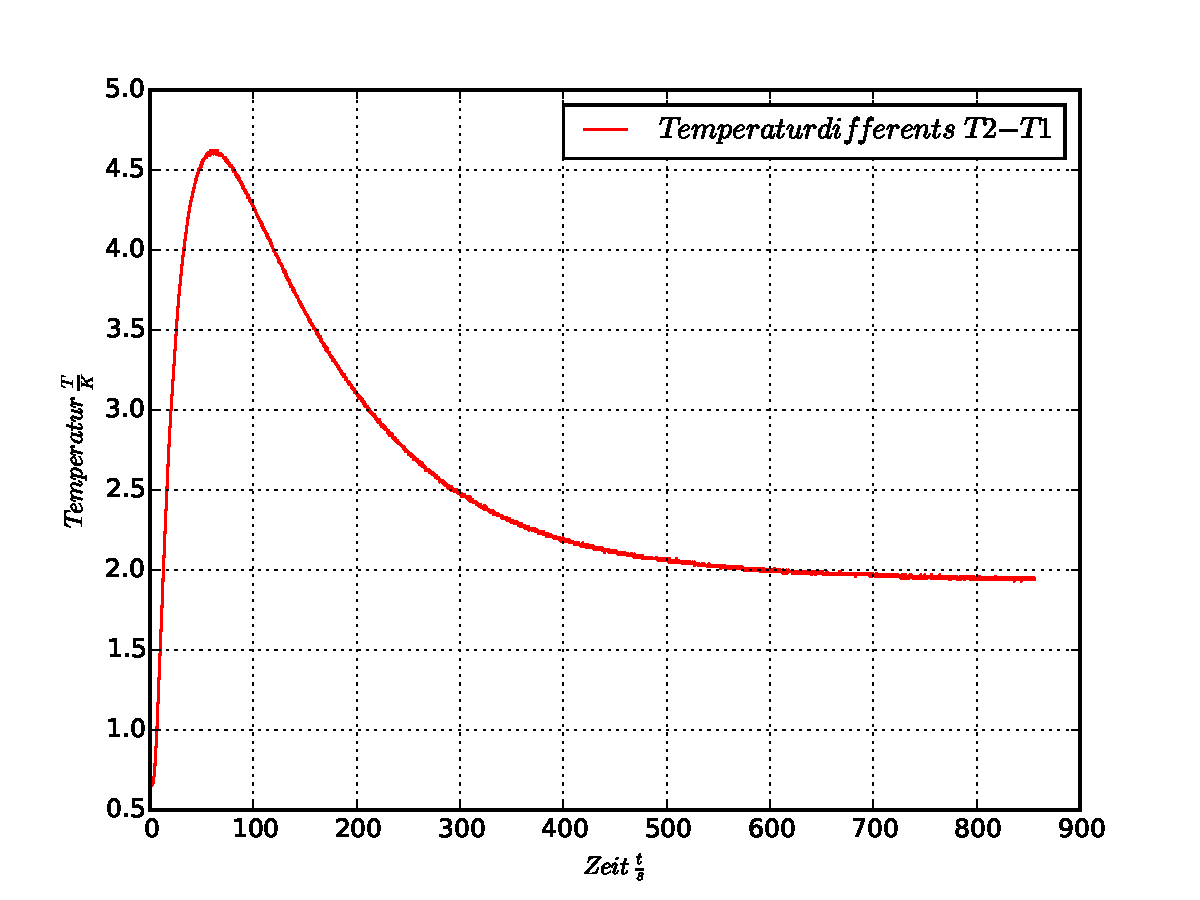
\includegraphics[width=0.7\textwidth]{plotT2-T1.pdf}
  \caption{Zeitahängige Temperaturdifferents zwischen $T_2$ und $T_1$.}
  \label{abb:T2-T1}
\end{figure}
\begin{figure}
  \centering
  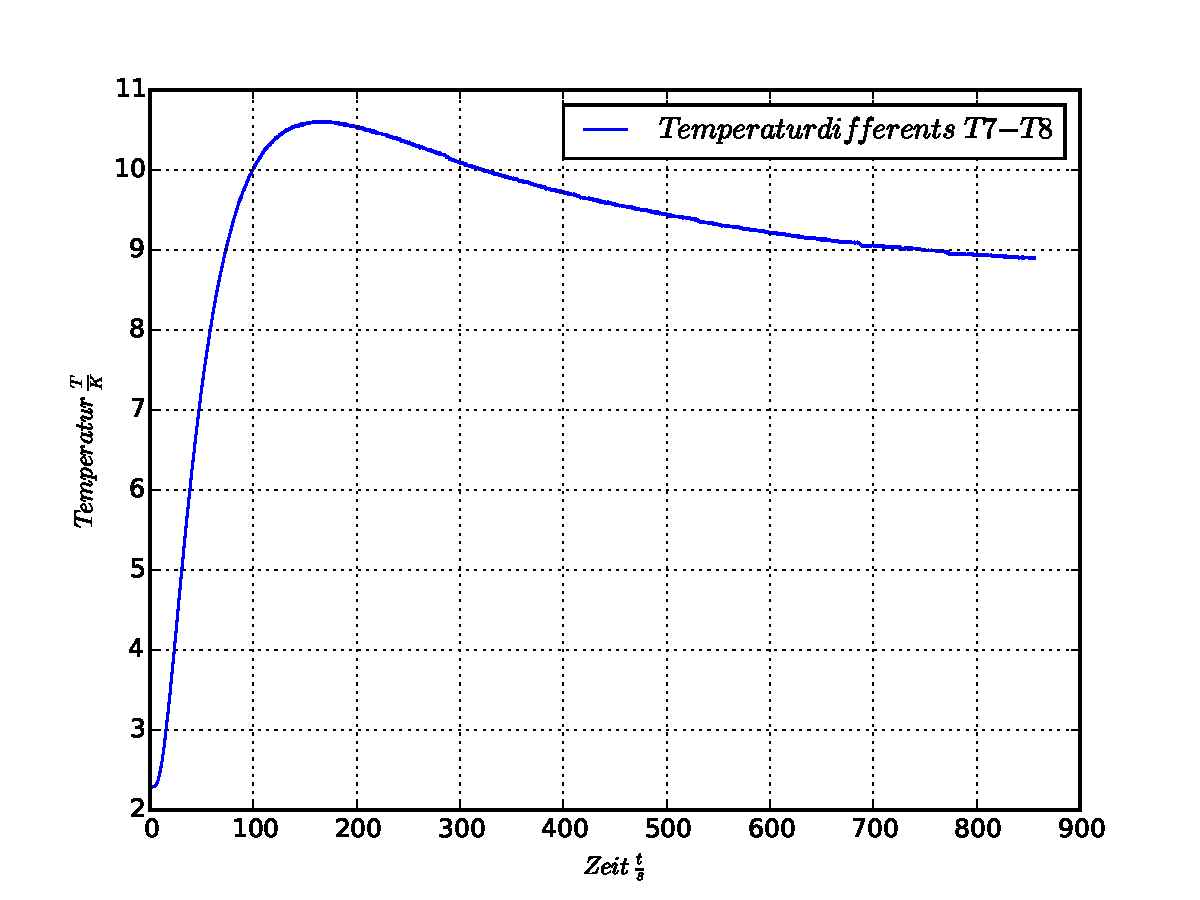
\includegraphics[width=0.7\textwidth]{plotT7-T8.pdf}
  \caption{Zeitahängige Temperaturdifferents zwischen $T_7$ und $T_8$.}
  \label{abb:T7-T8}
\end{figure}
Der Verlauf der Temperaturdifferenz der beiden Kurven
ist fast identisch. Die beiden Temperaturdifferenz begin am
Anfang stark zu steigen um danach wieder zu sinken
und langsam gegen eine konstante Temperaturdifferenz
zu konvergieren.
Der Unterschied zwischen den beiden Graphen besteht einmal
darin, dass bei der Kurve vom Stahl \ref{abb:T7-T8} die Endtemperaturdifferenz
deutlich höher ist als die von dem Messing \ref{abb:T2-T1}.


\subsection{Dynamische Methode}

Nun soll die Wärmeleitfähigkeit der einzelnen
Materialien durch
die Angström-Meßverfahren bestimmt werden.
In den Abbildung \ref{abb:T1T2},\ref{abb:T5T6} und \ref{abb:T7T8}
sind die gemessenen Temperaturwellen dargestellt.
\begin{figure}
  \centering
  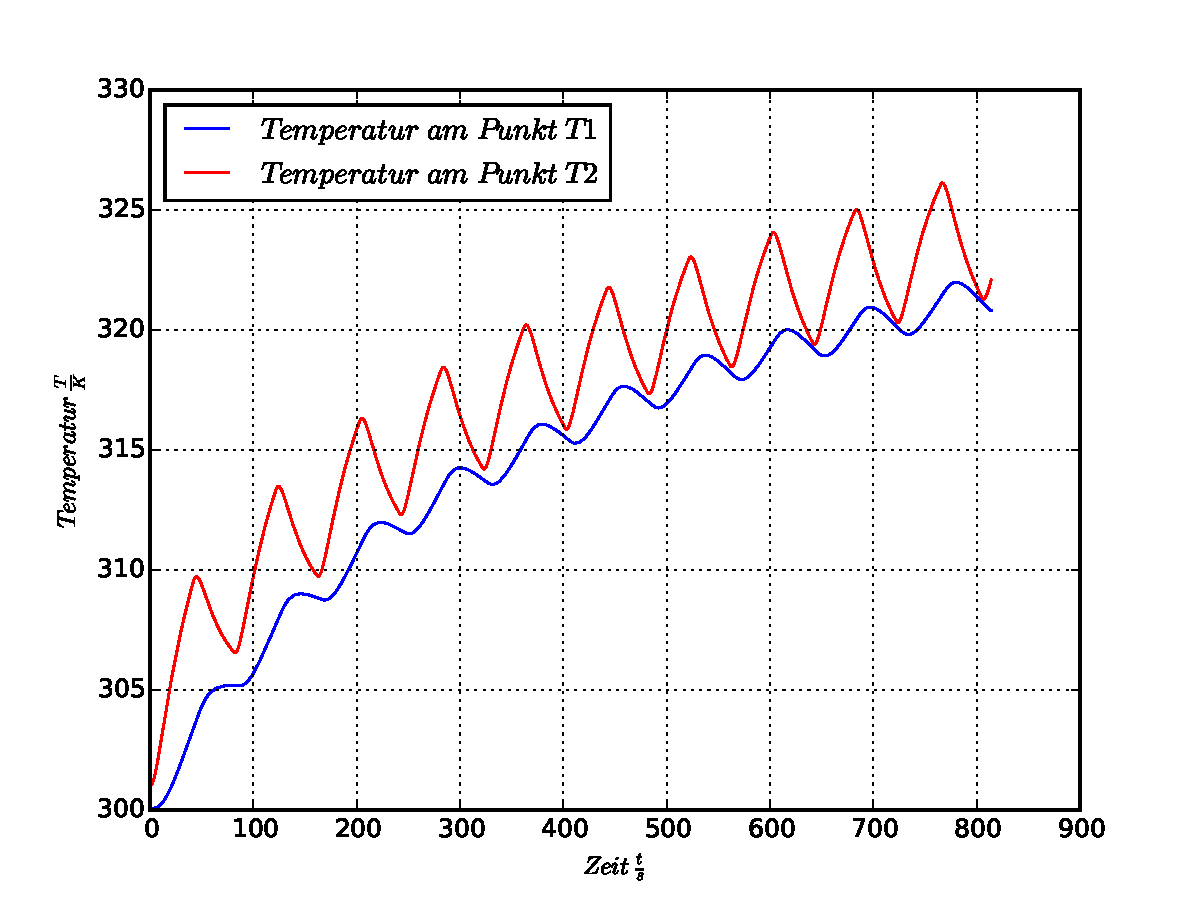
\includegraphics[width=0.7\textwidth]{plotT1T2.pdf}
  \caption{Temperaturverlauf an den Punkten $T_1$ und $T_2$.}
  \label{abb:T1T2}
\end{figure}
\begin{figure}
  \centering
  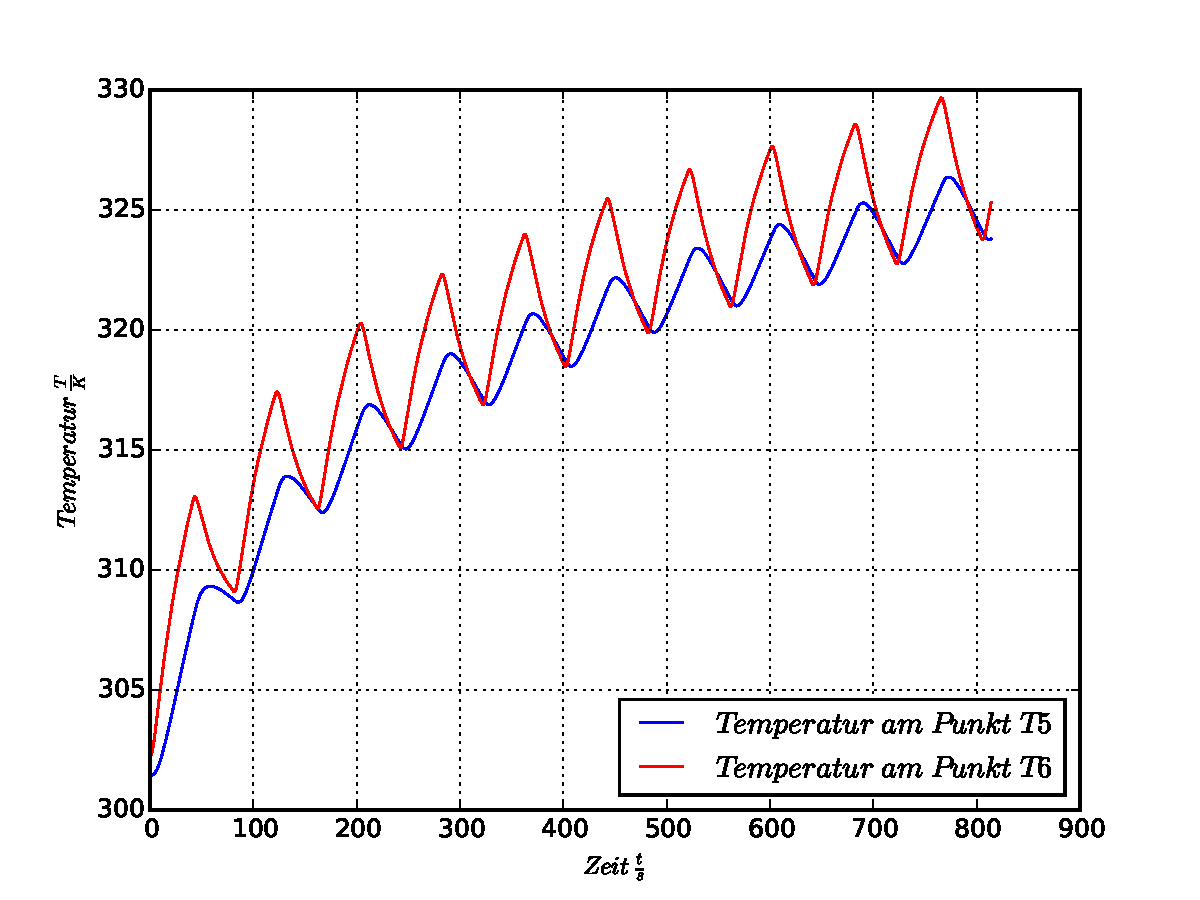
\includegraphics[width=0.7\textwidth]{plotT5T6.pdf}
  \caption{Temperaturverlauf an den Punkten $T_5$ und $T_6$.}
  \label{abb:T5T6}
\end{figure}
\begin{figure}
  \centering
  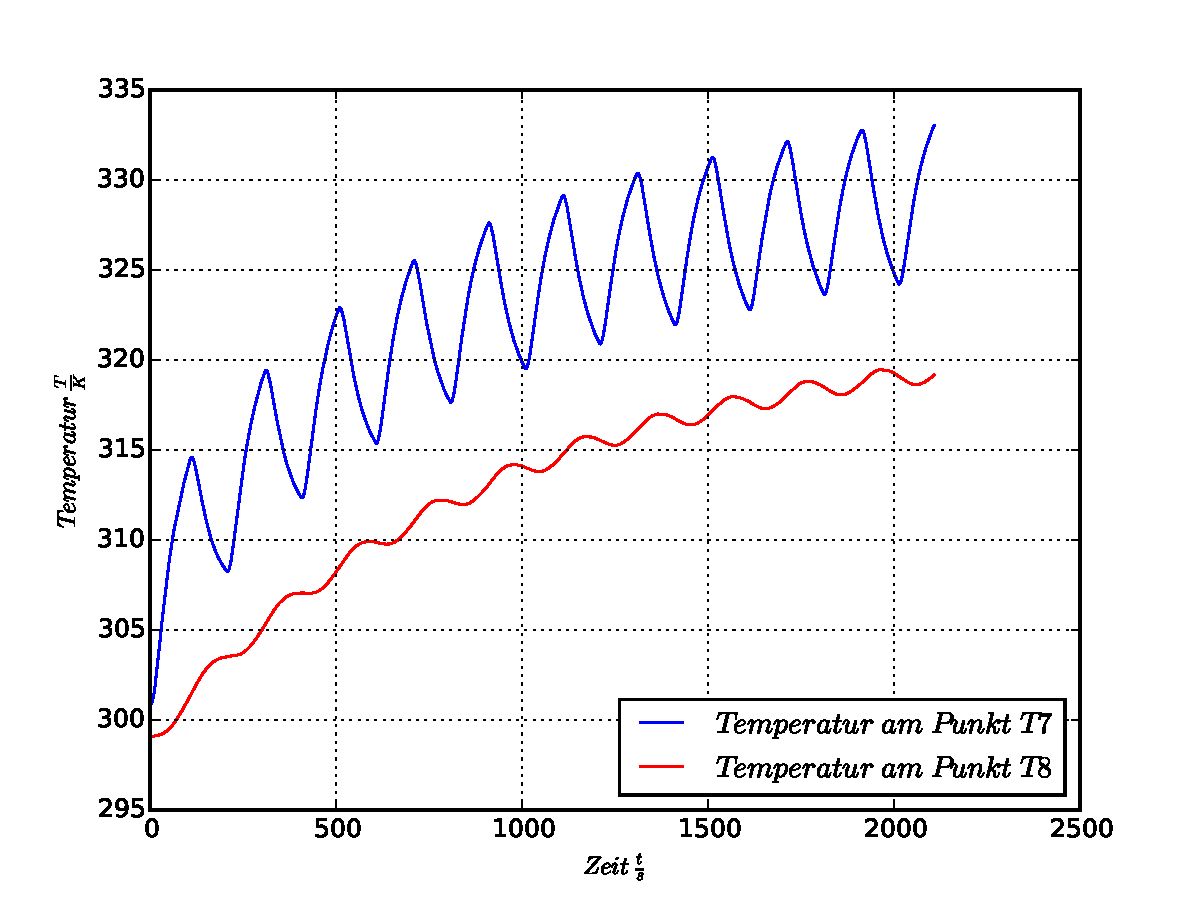
\includegraphics[width=0.7\textwidth]{plotT7T8.pdf}
  \caption{Temperaturverlauf an den Punkten $T_7$ und $T_8$.}
  \label{abb:T7T8}
\end{figure}
Die Wärmeleitfähigkeit berechent sich aus der Formel \eqref{eqn:k}.
Dafür werden mit Hilfe des Programm
PASCO Capstone die Exstremstellen
der einzelnen Kurven bestimmt und
die Amplituden mit Python nach der Formel
\begin{align}
A=\frac{T_\mathrm{hoch}-T_\mathrm{tief}}{2}
\end{align}
für die die einzeln Temperatwellen berechnet und gemittel.
Für die einzelnen Wellen ergibt sich somit:
\begin{align*}
A_\mathrm{T1}=& (0,38\pm0,19)\,\si{\kelvin}\\
A_\mathrm{T2}=& (2,14\pm0,24)\,\si{\kelvin}\\
A_\mathrm{T5}=& (1,04\pm0,28)\,\si{\kelvin}\\
A_\mathrm{T6}=& (2,69\pm0,28)\,\si{\kelvin}\\
A_\mathrm{T7}=& (4,05\pm0,24)\,\si{\kelvin}\\
A_\mathrm{T8}=& (0,23\pm0,13)\,\si{\kelvin}
\end{align*}
Ebenfalls muss zur Bestimmung der Wärmeleitfähigkeit
die Phasendifferenz $\Delta t$ bestimmt zwischen den Nahen-
und Fernewärmewellen bestimmt werden.
Hierfür wird die Zeit von den Extremstellen
der nahen
von dem fernen Thermoelementen abgezogen und
wieder gemittet werden.
Für $\Delta t$ zwischen $T_1$ und $T_2$ folgt somit
\begin{align*}
\Delta t_{12} &=(12,5\pm3,6)\,\si{\second}
\intertext{Zwischen $T_5$ und $T_6$}
\Delta t_{56} &=(7,1\pm1,3)\,\si{\second}
\intertext{und zwischen $T_7$ und $T_8$}
\Delta t_{78} &= (51,9\pm13,1)\,\si{\second}
\end{align*}
Der Abstand zwischen alles Messstellen berträgt:
\begin{align*}
\Delta x = 0,03\,\si{\meter}
\end{align*}
Die notwendige Dichte $\rho$ und die speziefische
Wärmekapazität $c$ der einzelen Materialien wird aus
der Tabelle \ref{tab:crho} genommen.
\begin{table}
  \centering
  \caption{}
  \label{tab:crho}
  \begin{tabular}{c c c c}
    \toprule
    Material & $Diche \rho/\si{\kilo\gram\per\meter\tothe{2}}  $ &  spe. Wärmekapazität $c/\si{\joule\per\kilo\gram\kelvin}$ \\
    \midrule
    Messing   &  8520  & 385\\
    Aluminium &  2800  & 830\\
    Edelstahl &  8000  & 400\\
    \bottomrule
  \end{tabular}
\end{table}

Durch einsetzen all dieser Werte in die
Formel \eqref{eqn:k}
ergeben sich die Wärmeleitfähigkeiten von:
\begin{align*}
\intertext{Messing:}
\kappa_\mathrm{Messing}  =&(68\pm28)\,\si{\watt\per\meter\kelvin}
\intertext{Aluminium:}
\kappa_\mathrm{Aluminium}=&(160\pm60)\,\si{\watt\per\meter\kelvin}
\intertext{Edelstahl:}
\kappa_\mathrm{Edelstahl}=&(10\pm3)\,\si{\watt\per\meter\kelvin}
\end{align*}
Mit Hilfe der Formel \eqref{eqn:abweich} lässt sich die
relative Abweichungen von den Literaturwerte berechen.
\begin{align*}
\intertext{Die Abweichung für Messing beträgt:}
a_\mathrm{messing}=16\,\si{\percent}
\intertext{Für Aluminium:}
a_\mathrm{messing}=22\,\si{\percent}
\intertext{Für Edelstahl:}
a_\mathrm{messing}=51\,\si{\percent}
\end{align*}
